\documentclass{beamer}

\usepackage{tikz}
\usetikzlibrary{positioning,matrix}
\usepackage{blindtext}
\usepackage{graphicx}

\graphicspath{{./img}}

\usetheme{Madrid}

\title{Federate Orchestration for Cloud-Fog Infrastructure}
%\subtitle{What is Dominic working on?}
\author{Dominic Lindsay}
\institute{Lancaster Univeristy}
%\date{}

\begin{document}
	
	\frame{\titlepage}
	
	\section{Introduction}
	\begin{frame}
		\frametitle{Overview}
		\framesubtitle{Todays Presentation...}
		\begin{itemize}
			\item Introduction
			\item \textit{Fog-Cloud Computing}
			\item Orchestration at the edge
			\item Quality of Service
			\item Problem Statement
			\item Proposal
			\item System Design
			\item HotCloud'20 
			\item Questions
%			\item References
		\end{itemize}
	\end{frame}

\section{Cloud-Fog Computing}
\begin{frame}
	\frametitle{Cloud-Fog Computing}
	\framesubtitle{\textit{Cloud-Fog Continuum}}
	\begin{columns}[T] % contents are top vertically aligned
		\column{.5\textwidth} % column designated by a command
		\begin{block}{Hierarcichal Network}
			\begin{itemize}
				\item \textit{Cloud-Fogs} are composed of hierarchal networks.
				\item Nodes top possess more \textit{resources} and exhibit higher \textit{availability}.
			\end{itemize}
		\end{block}
		\begin{block}{Characteristics}
			\begin{enumerate}
				\item Distributed Infrastructure
				\item Non-Neglible Latencies
				\item Limited Availability and Reachability
			\end{enumerate}
			
		\end{block}

		\column{.5\textwidth}
		\begin{figure}
			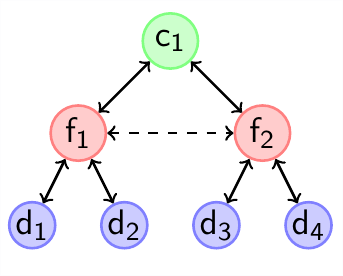
\includegraphics[height=3cm]{img/cloud-fog.png}
			\caption{\centering Cloud-Fog Network. Cloud Clusters possessing the most resources are found at the top with high availability, whilst Fog Node/Cloudlets are in middle tier, posess less resources but possess lower latencies and higher aggregate bandwidth.}
		\end{figure}	
\end{columns}
\end{frame}

\section{Orchestration}
\begin{frame}
	\frametitle{Orchestration}
	\framesubtitle{Autonomous Resource Management and Workload Execution}
	\begin{itemize}
		\item Orchestration
		\begin{itemize}
			\item Scheduling and Resource Management
			\item Cloud Orchestration
		\end{itemize}
	\end{itemize}
\end{frame}



\begin{frame}
	\frametitle{Application Contexts}
	\framesubtitle{\textit{Applications DAGs}}
%	\begin{columns}[T] % contents are top vertically aligned
%		\column{.5\textwidth} % column designated by a command
\begin{block}{Application DAG}
		\begin{itemize}
			\item Application submit jobs as DAGs.
			\item Vertices identify tasks and their requirements \\ \textit{e.g. spark executor $\langle$2GB, 1CPU$\rangle$}
			\item Edges identify both \textit{time and space} constraints.
			\item Task are executed by workers on behalf of an \textit{Application Master}.
			\item \textit{or clusters}
		\end{itemize}
\end{block}
%		\column{.5\textwidth}
\begin{exampleblock}{Example \textit{DAG}}
		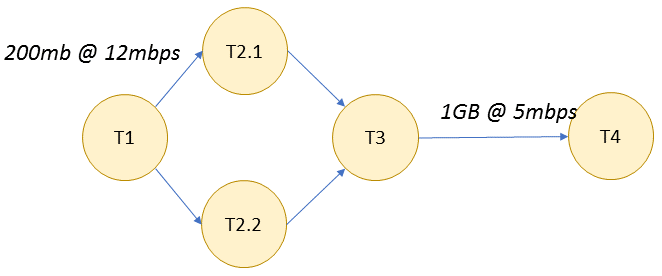
\includegraphics[height=2.5cm]{img/task-dag.png}
	\end{exampleblock}
%	\end{columns}
\end{frame}


\section{Quality of Service}
	\begin{frame}		
	 	\frametitle{Quality of Service}
		\begin{block}{Application Performance}
			Applications are composed of individual services\\
			Workers execute work on behalf of Application Masters\\
		\end{block}
		\begin{alertblock}{Intra-Service Quality of Service}
			\begin{itemize}
				\item Application depends on multiple services for execution of tasks.
				\item Intra-Node \textit{Bandwidth} and \textit{Latency} dictates \textit{QoS} of task executors.
			\end{itemize}
		\end{alertblock}
	\end{frame}

\section{Problem Statement}
	\begin{frame}
		\frametitle{Fog-Cloud Orchestration}
		\begin{block}{Centralised Orchestration}
			Orchestration Systems typically manage only a single cluster.\\
			As such resources are manage as a single flat hierarchy.\\
		\end{block}
	
		\begin{alertblock}{False Assumptions}
			Centralised orchestration systems exhibit several limitations when managing \textit{Cloud-Fogs} 
			\begin{itemize}
				\item Non-Negligible Intra-Cluster Latencies
				\item Unlimited intra-cluster bandwidths
				\item Uniform Sub-Cluster Resource Utilization
				\item Uniform Sub-Cluster Workload Affinity
			\end{itemize}
		\end{alertblock}
	
		\begin{alertblock}{\centering \textbf{Leading to poor quality placement and degraded application performance}}
%			\begin{itemize}
%				\item 
%			\end{itemize}
		\end{alertblock}
	\end{frame}

\section{Proposal}
\begin{frame}
	\frametitle{Proposal}
	\framesubtitle{Federate Orchestration Framework}
	\begin{block}{Hierarchical Resources}
		Fog-Cloud computing require orchestration
mechanisms capable of adapting to dynamic
sub-cluster 
		utilization and dynamic bandwidth
and latency constraints.
	\end{block}

	\begin{alertblock}{Objective}
		The objective of this work is to investigate new orchestration mechanisms for resource management in 
		decentralised Cloud-Fogs infrastructures, capable of making \textit{QoS} aware placements in dynamic hierarchical infrastructures. 
	\end{alertblock}

	\begin{exampleblock}{Contributions}
		\begin{itemize}
			\item Two-Layer Federate, Mobility Aware Orchestration Platform
			\item Bandwidth and Latency Migration Policy
			\item High Level Application Level Constraints.
		\end{itemize}
	\end{exampleblock}
\end{frame}
%\section{Application Aware Scheduling}


\section{System Design}
\begin{frame}
	\frametitle{Requirements}
	\begin{block}{Cluster Aware}
		Workload posses affinities to differnt scheduling archetectures\\
		Cluster Utilization impacts workload performance
	\end{block}
	\begin{block}{\textit{Quality of Service Aware}}
		Quality of Service is dictated not only by resource (CPU, mem, etc) but by bandwidth and latency across sub-clusters
	\end{block}
	\begin{block}{Application Aware}
		Careful placement of a workload can lead to increased performance.\\
		Scheduler should be aware of executor population.\\
		Provide Cluster Affinity/Anti-Affinity and Cardinality.
	\end{block}
\end{frame}

\begin{frame}
	\frametitle{System Diagram}
	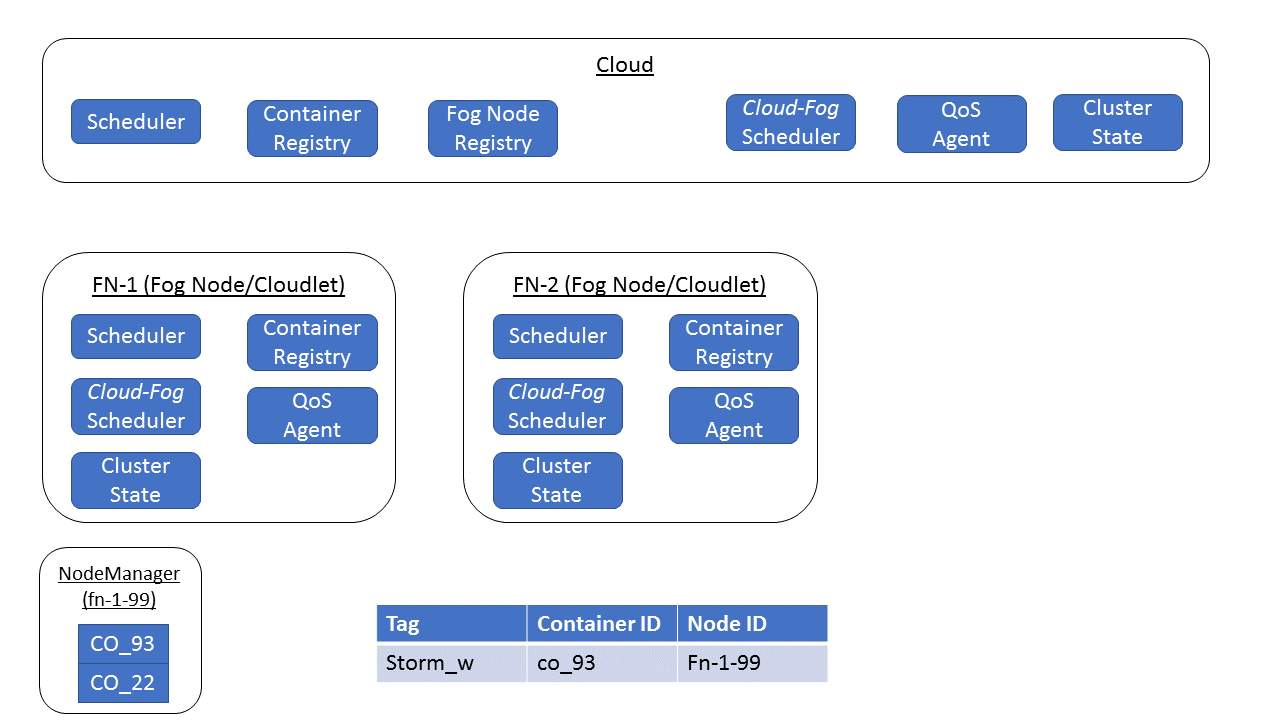
\includegraphics[height=.85\textheight,width=\textwidth]{img/system_diagram}
\end{frame}


\section{HotCloud'20}
\begin{frame}
	\frametitle{HotCloud'20}
	\begin{itemize}
		\item USENIX workshop
		\item Fancy Companies
		\item Deadline: 17th March
	\end{itemize}
\end{frame}

\section{Questions}
\begin{frame}
	\centering Questions?	
\end{frame}
\end{document}
